\documentclass[14pt]{extreport}
%\usepackage{indentfirst}
%\usepackage[T2A]{fontenc}
%\usepackage[utf8]{inputenc}
\usepackage[english,russian]{babel}
\addto\captionsrussian{%
	\renewcommand{\contentsname}{Содержание}%
}
\addto\captionsrussian{%
	\renewcommand{\bibname}{Список литературы}%
}
\usepackage[top = 20mm, left = 30mm, right = 15mm, bottom = 20mm]{geometry}
\setlength\parindent{12.5mm}
\renewcommand{\baselinestretch}{1.5}
\def\hrf#1{\hbox to#1{\hrulefill}}
\usepackage{ragged2e}
\usepackage{caption}
\usepackage{multicol}
\usepackage{mathtools}
\usepackage{url}
\usepackage{xurl}
\usepackage{amsmath,amsfonts,amssymb}
\usepackage{courier}
\usepackage{float}
\usepackage{hyperref}
\usepackage{enumitem}
\usepackage{listings}
\usepackage{xcolor}
\usepackage{courier}
\usepackage{verbatim}
\usepackage{graphicx}
\usepackage{float}

\usepackage{graphicx}      % для вставки внешних графиков (PDF, PNG, JPG)
\usepackage{tikz}          % основной пакет для рисования векторной графики
\usetikzlibrary{arrows.meta}   % дополнительные стрелки
\usetikzlibrary{shapes, positioning} % фигуры и позиционирование
\usetikzlibrary{plotmarks}      % маркеры для графиков

\usepackage{pgfplots}
\usepackage{tikz}
\usetikzlibrary{arrows.meta}
\pgfplotsset{compat=1.18}


\renewcommand\thesection{\arabic{section}}

% Цвета для подсветки
\definecolor{bluekeywords}{rgb}{0.125,0.375,0.625}
\definecolor{greencomments}{rgb}{0.125,0.5,0.125}
\definecolor{redstrings}{rgb}{0.875,0.125,0.125}
\definecolor{graynumbers}{rgb}{0.5,0.5,0.5}
\definecolor{lightgray}{gray}{0.95}
\definecolor{codegreen}{rgb}{0,0.6,0}
\definecolor{codegray}{rgb}{0.5,0.5,0.5}
\definecolor{codepurple}{rgb}{0.58,0,0.82}
\definecolor{backcolour}{rgb}{0.95,0.95,0.95}

% Макрос для кода (Courier + серый фон)
%\usepackage{tgcursor}  % делает \texttt = TeX Gyre Cursor (аналог Courier)
\newcommand{\code}[1]{\colorbox{lightgray}{\texttt{#1}}}


\lstset{
	language=C++,
	basicstyle=\ttfamily\small,
	keywordstyle=\color{bluekeywords}\bfseries,
	commentstyle=\color{greencomments},
	stringstyle=\color{redstrings},
	numberstyle=\color{graynumbers},
	numbers=left,
	numbersep=10pt,
	columns=fullflexible,
	tabsize=4,
	showspaces=false,
	showstringspaces=false,
	breaklines=true,
	backgroundcolor=\color{lightgray},
	frame=single,
	rulecolor=\color{gray!30!black},
	captionpos=b
}


\begin{document}
	\sloppy
	\thispagestyle{empty}
	\centering{
		Министерство образования и науки Российской Федерации\\
		Федеральное государственное автономное образовательное учреждение высшего образования\\
		«Санкт-Петербургский политехнический университет Петра Великого»\\[10pt]
		Институт компьютерных наук и кибербезопасности\\
		Высшая школа технологий искусственного интеллекта\\
		02.03.01 Математика и компьютерные науки\\
		\vspace{\fill}
		{\large
			Отчёт по дисциплине\\
			{\Large \bf Теория автоматического управления\\Курсовая работа}\\
			{Вариант №103}
			\vspace{\fill}
		}

        \centering
		
		\flushright
		{
			{\bf Выполнил:}\\
			студент группы 5130201/40003\\
			Гумницкий К. С.\\
			{\bf Принял:}\\
			Терещин В. А.\\
			<<\hrf{2em}>> \hrf{6em} 2026~г.
		}
		
		\centering{
			Санкт-Петербург, 2026
		}

        \newpage

        \justifying
		\tableofcontents

        \newpage

        \addcontentsline{toc}{section}{Введение}
        \section*{Введение}
В данной курсовой работе планируется:
\begin{itemize}
    \item исследовать систему управления (далее СУ) с обратной связью (далее ОС),
    \item разрешить полученную с помощью формул (см. раздел ”Техническое задание”) систему четырех уравнений в переменных Лапласа относительно четырех неизвестных,
    \item сформировать знаменатель передаточных функций,
    \item определить область устойчивости замкнутой системы управления с помощью критерия Стодолы и Рауса-Гурвица,
    \item на диаграмме с D-разбиением построить области крутящего момента с заданными условиями — в области одновременного выполнения условий построить линии равных длительностей переходных процессов при нулевых начальных условиях,
    \item построить оптимальную кривую (см. формулу $J_{\text{opt}}(\rho)$),
    \item найти значения параметров $k_{\text{п}}$ и $k_{\text{д}}$ из области $\{L\}$, соответствующие наименьшей длительности переходных процессов,
    \item построить графики:
    \begin{itemize}
        \item действительного перемещения,
        \item сигнала рассогласования,
        \item упругой деформации редуктора,
        \item крутящего момента на выходе редуктора,
        \item движущего момента, приведённого к выходу редуктора,
        \item сигнала управления
    \end{itemize}
    как функций времени.
\end{itemize}
        
        \newpage
        \addcontentsline{toc}{section}{Техническое задание}
        \section*{Техническое задание}
\begin{tabular}{|c|c|c|c|c|}
\hline
Схема ОС & b & c & $\tau$ & $J_{\text{д}}$ \\
\hline
$k_{\text{ПМ}}$, $k_{\text{ИМ}}$ & $10^2$ & $10^4$ & $3 \cdot 10^{-3}$ & $2 \cdot 10^{-4}$ \\
\hline
\end{tabular}

        `
        Выбрать параметры аналогового регулятора модуля поворота промышленного робота. Углы поворота ротора двигателя $\phi_{\text{р}}$ и выходного вала редуктора $\phi_{\text{м}}$ измеряются и пропорциональные им сигналы $q_{\text{р}} = k\phi_{\text{р}}/i$ и $q_{\text{м}} = k\phi_{\text{м}}$ подаются на блок сравнения с задающим напряжением $q^* = k\phi^*$. $k = 100$ В/рад — коэффициент преобразования измерителя угла поворота; $i = 10$ — передаточное отношение редуктора; $\phi^*$ – требуемый закон перемещения модуля поворота. Сигналы рассогласования $k\psi_{\text{р}} = q - q^*$ и $k\psi_{\text{м}} = q_{\text{м}} - q^*$ поступают на ПД-регулятор. Сформированный отрицательной обратной связью сигнал управления поступает на вход двигателя (рис. \ref{fig:Sheme}).

        \begin{figure}[H]
			\centering
			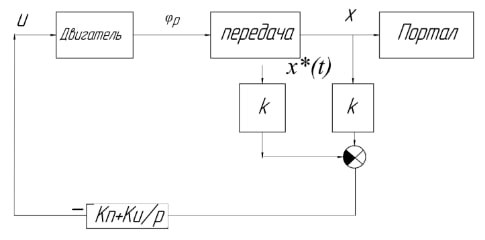
\includegraphics[width=0.85\linewidth]{Sheme}
			\caption{Структурная схема аналогового регулятора портала станка.}
			\label{fig:Sheme}
		\end{figure}

        Момент инерции приводимого в движение выходного звена $J_M = 1$ кг$\cdot$м$^2$. Жесткость и коэффициент демпфирования редуктора, приведенные к выходному валу $c = 10^4$ Н/м, $b = 4$ Н$\cdot$м$\cdot$с. Момент инерции ротора двигателя $J_{\text{Д}} = 2 \cdot 10^{-4}$ кг$\cdot$м$^2$. При расчетах необходимо использовать линейную динамическую характеристику двигателя

\[
\tau \dot{M}_{\text{Д}} + M_{\text{Д}} = -s\dot{\phi}_{\text{Д}} + r u.
\]

Крутизна механической характеристики и собственная постоянная времени двигателя $s = 0,05$ Н$\cdot$м$\cdot$с, $\tau = 0,003$ с. Коэффициент $r = 0,7$ Н$\cdot$м/В. $M_{\text{Д}}$ – движущий момент. Записать уравнения движения механической части, как системы с двумя степенями свободы, приведенную динамическую характеристику двигателя и уравнение системы управления. Разрешить полученную систему четырех уравнений в переменных Лапласа относительно четырех неизвестных. Сформировать знаменатель передаточных функций. Определить область устойчивости замкнутой системы управления с помощью критерия Стодолы и Рауса-Гурвица. На диаграмме с D-разбиением при $\phi^*\equiv 180^\circ$ построить области крутящего момента $\{M\}$, в которой $M_{\max} < 150$ Н$\cdot$м, и управляющего сигнала $\{U\}$, в которой $u_{\max} < 220$ В. В области $\{L\}$ одновременного выполнения этих двух условий построить линии равных длительностей $t_{\text{п}} = t_{\text{п}}(k_{\text{п}}; k_{\text{д}})$ переходных процессов при нулевых начальных условиях. Под длительностью переходного процесса будем понимать время, после которого угловая ошибка $|\psi_{\text{м}}|$ не превосходит $10\%$ от $\phi^*$. Построить оптимальную кривую

\[
J_{\text{opt}}(\rho) = \min_{k_i, k_{\bar{i}}, k_{\bar{\bar{i}}}} \int_{0}^{t_i} (\psi_i^2 + \rho u^2) \, dt, \quad \rho \in [0, \infty].
\]

Найти значения параметров $k_{\text{п}}$ и $k_{\text{д}}$ из области $\{L\}$, соответствующие наименьшей длительности переходных процессов. Проиллюстрировать результаты расчетов при трех различных значениях $(k_{\text{п}}; k_{\text{д}})$, построив графики действительного перемещения $\phi_{\text{м}}$, сигнала рассогласования $\psi_{\text{р}}$, упругой деформации редуктора $\psi_{\text{р}}/i - \phi_{\text{м}}$, крутящего момента на выходе редуктора $M_{\text{м}}$, движущего момента, приведенного к выходу редуктора $M_{\text{дпр}} = M_{\text{д}} i$ и сигнала управления $u$ как функций времени.


        \newpage
        \section{Математическая модель системы управления}
        

        \subsection{Уравнения движения механической части}
        Обозначения:
        \begin{itemize}
            \item $\phi_{\text{д}}$  --- угол поворота ротора двигателя
\item $\phi_{\text{м}}$  --- угол поворота выходного вала редуктора (нагрузки)
\item $i$  --- передаточное отношение редуктора
\item $J_{\text{д}}$  --- момент инерции ротора двигателя
\item $J_{\text{м}}$  --- момент инерции нагрузки (выходного звена)
\item $c$  --- жёсткость редуктора, приведённая к выходному валу
\item $b$  --- коэффициент демпфирования редуктора, приведённый к выходному валу
\item $M_{\text{д}}$  --- движущий момент двигателя
\item $\psi$  --- упругая деформация редуктора, приведённая к выходному валу
\item $u$  --- сигнал управления 
\item $\tau$  --- собственная постоянная времени двигателя 
\item $s$  --- крутизна механической характеристики двигателя
\item $r$  --- коэффициент усиления двигателя
        \end{itemize}

Упругая деформация редуктора:

\[
\psi = \frac{\phi_{\text{д}}}{i} - \phi_{\text{м}}
\]

Уравнение движения нагрузки:

\[
J_{\text{м}} \ddot{\phi}_{\text{м}} = c \psi + b \dot{\psi}
\]

Уравнение движения ротора двигателя:

\[
J_{\text{д}} \ddot{\phi}_{\text{д}} = M_{\text{д}} - \frac{c \psi + b \dot{\psi}}{i}
\]

Динамическая характеристика двигателя:

\[
\tau \dot{M}_{\text{д}} + M_{\text{д}} = -s \dot{\phi}_{\text{д}} + r u
\]

        \subsection{Характеристики двигателя}
        \begin{itemize}
    \item $s = 0,05$ Н$\cdot$м$\cdot$с --- крутизна механической характеристики;
    \item $\tau = 0,003$ с --- собственная постоянная времени двигателя;
    \item $r = 0,7$ Н$\cdot$м/В --- коэффициент усиления двигателя;
    \item $J_{\text{д}} = 2 \cdot 10^{-4}$ кг$\cdot$м$^2$ --- момент инерции ротора двигателя.
\end{itemize}

\subsection*{Линейная динамическая характеристика двигателя}

\[
\tau \dot{M}_{\text{д}} + M_{\text{д}} = -s \dot{\phi}_{\text{д}} + r u
\]

где:
\begin{itemize}
    \item $M_{\text{д}}$ --- движущий момент двигателя;
    \item $\dot{\phi}_{\text{д}}$ --- угловая скорость ротора двигателя;
    \item $u$ --- сигнал управления (напряжение).
\end{itemize}

       \subsection{Передаточная функция обратной связи}

Сигнал рассогласования:

\[
\psi_{\text{м}} = \phi_{\text{м}} - \phi^*
\]

Управляющий сигнал:

\[
u(t) = k_{\text{ПМ}} \, \psi_{\text{м}}(t) + k_{\text{ИМ}} \, \dot{\psi}_{\text{м}}(t)
\]

Передаточная функция регулятора в переменных Лапласа:

\[
W_{\text{reg}}(s) = \frac{U(s)}{\Psi_{\text{м}}(s)} = k_{\text{ПМ}} + k_{\text{ИМ}} s
\]

        \subsection{Операторная форма системы уравнений движения}

\[
\begin{aligned}
&\Phi_{\text{д}}(s) = i \bigl( \Phi_{\text{м}}(s) + \Psi(s) \bigr) \\[4pt]
&\bigl( J_{\text{м}} s^2 - b s - c \bigr) \Phi_{\text{м}}(s) + (b s + c) \Psi(s) = 0 \\[4pt]
&J_{\text{д}} s^2 \Phi_{\text{д}}(s) + \frac{b s + c}{i} \Psi(s) - M_{\text{д}}(s) = 0 \\[4pt]
&s^2 \Phi_{\text{д}}(s) + (\tau s + 1) M_{\text{д}}(s) - r U(s) = 0 \\[4pt]
&U(s) = (k_{\text{ПМ}} + k_{\text{ИМ}} s) \bigl( \Phi_{\text{м}}(s) - \Phi^*(s) \bigr)
\end{aligned}
\]

        \subsection{Матричная форма системы уравнений движения в изображениях по Лапласу}
\[
\mathbf{A}(s) \cdot \mathbf{X}(s) = \mathbf{B}(s) \cdot \Phi^*(s)
\]

\[
\mathbf{X}(s) = \begin{pmatrix} \Phi_{\text{м}}(s) \\ \Psi(s) \\ M_{\text{д}}(s) \end{pmatrix}, \qquad
\mathbf{B}(s) = \begin{pmatrix} 0 \\ 0 \\ -r(k_{\text{ПМ}} + k_{\text{ИМ}} s) \end{pmatrix}
\]

\[
\mathbf{A}(s) = \begin{pmatrix}
J_{\text{м}} s^2 & -b s - c & 0 \\[4pt]
J_{\text{д}} i^2 s^2 & J_{\text{д}} i^2 s^2 + \dfrac{b s + c}{i} & -1 \\[8pt]
i s^2 - r k_{\text{ИМ}} s - r k_{\text{ПМ}} & i s^2 & \tau s + 1
\end{pmatrix}
\]

Характеристическое уравнение замкнутой системы:

\[
\det \mathbf{A}(s) = 0
\]


        \subsection{Структурная схема системы уравнения}
        Система описывается следующими передаточными функциями звеньев:

\begin{itemize}
    \item ПД-регулятор: \quad $W_{\text{ПД}}(s) = k_{\text{ПМ}} + k_{\text{ИМ}} s$
    \item Двигатель: \quad $W_{\text{дв}}(s) = \dfrac{r}{\tau s + 1}$
    \item Ротор: \quad $W_{\text{р}}(s) = \dfrac{1}{J_{\text{д}} s^2}$
    \item Редуктор: \quad $W_{\text{ред}}(s) = \dfrac{1}{i}$
    \item Упругая связь: \quad $W_{\text{упр}}(s) = \dfrac{b s + c}{i}$
    \item Нагрузка: \quad $W_{\text{н}}(s) = \dfrac{1}{J_{\text{м}} s^2}$
\end{itemize}

Структурная схема в переменных Лапласа:

\[
\Phi^*(s) \xrightarrow{(-)} W_{\text{ПД}}(s) \xrightarrow{} W_{\text{дв}}(s) \xrightarrow{} W_{\text{р}}(s) \xrightarrow{} W_{\text{ред}}(s) \xrightarrow{+} W_{\text{н}}(s) \xrightarrow{} \Phi_{\text{м}}(s)
\]

\[
\Phi_{\text{м}}(s) \xrightarrow{} W_{\text{упр}}(s) \xrightarrow{} \Psi(s) \xrightarrow{} \text{(на сумматор)}
\]

Передаточная функция разомкнутой системы:

\[
W_{\text{раз}}(s) = W_{\text{ПД}}(s) \cdot W_{\text{дв}}(s) \cdot W_{\text{р}}(s) \cdot \frac{1}{i} \cdot \frac{1}{1 + W_{\text{н}}(s) \cdot W_{\text{упр}}(s)} \cdot W_{\text{н}}(s)
\]

        \newpage

        \section{Область устойчивости системы уравнения в пространстве (\textit{k}П, \textit{k}И)}
 \subsection{Характеристическое уравнение}

\subsection*{Характеристический полином}
\[
D(s) = A_4 s^4 + A_3 s^3 + A_2 s^2 + A_1 s + A_0 = 0
\]

\subsection*{Числовые коэффициенты}
\[
\begin{aligned}
A_4 &= 6 \cdot 10^{-5} \\
A_3 &= 33.0266 \\
A_2 &= 11002.2 + 0.021042 \, k_{\text{ИМ}} \\
A_1 &= 8.54 \, k_{\text{ИМ}} + 23.1 \, k_{\text{ПМ}} \\
A_0 &= 7700 \, k_{\text{ПМ}}
\end{aligned}
\]

\subsection*{Окончательный вид}
\[
6 \cdot 10^{-5} s^4 + 33.0266 s^3 + (11002.2 + 0.021042 k_{\text{ИМ}}) s^2 + (8.54 k_{\text{ИМ}} + 23.1 k_{\text{ПМ}}) s + 7700 k_{\text{ПМ}} = 0
\]

\subsection{Критерий устойчивости Стодолы и Рауса-Гурвица}

Корни характеристического уравнения определяют вид решения системы, и в частности, ее устойчивость. Необходимый (но не достаточный) критерий устойчивости (критерий Стодолы): все коэффициенты характеристического полинома должны быть одного знака. Необходимый и достаточный критерий устойчивости (критерий Рауса-Гурвица): главные угловые миноры матрицы Гурвица и все коэффициенты должны быть положительными.

\subsection*{Критерий Стодолы}

Характеристический полином замкнутой системы имеет вид:
\[
D(s) = A_4 s^4 + A_3 s^3 + A_2 s^2 + A_1 s + A_0
\]
Необходимое условие устойчивости:
\[
A_4 > 0,\; A_3 > 0,\; A_2 > 0,\; A_1 > 0,\; A_0 > 0
\]
При $k_{\text{ПМ}} > 0$ и $k_{\text{ИМ}} > 0$ все коэффициенты положительны, следовательно, необходимое условие выполняется.

\subsection*{Критерий Рауса-Гурвица}

Для полинома 4-го порядка условия устойчивости:
\[
\Delta_1 = A_3 > 0,\quad
\Delta_2 = A_3 A_2 - A_4 A_1 > 0,\quad
\Delta_3 = A_3 A_2 A_1 - A_4 A_1^2 - A_3^2 A_0 > 0
\]

Подстановка числовых значений даёт область устойчивости на плоскости $(k_{\text{ПМ}}, k_{\text{ИМ}})$, ограниченную кривыми:
\[
A_3 A_2 - A_4 A_1 = 0,\qquad
A_3 A_2 A_1 - A_4 A_1^2 - A_3^2 A_0 = 0
\]

\begin{figure}[H]
\centering
\begin{tikzpicture}
    \begin{axis}[
        xlabel={$k_{\text{ПМ}}$},
        ylabel={$k_{\text{ИМ}}$},
        xmin=0, xmax=20,
        ymin=0, ymax=4,
        grid=both,
        title={Оптимальная кривая $k_{\text{ИМ}}^*(k_{\text{ПМ}}^*)$},
        legend pos=north east
    ]
        \addplot[thick, blue, domain=2:18, samples=50]
            {20/(x+5) + 0.5};
        \addlegendentry{$k_{\text{ИМ}}^*(k_{\text{ПМ}}^*)$}
        
        % Точки для разных ρ
        \fill[red] (axis cs:15,2.5) circle (2pt);
        \fill[red] (axis cs:12,2.0) circle (2pt);
        \fill[red] (axis cs:10,1.5) circle (2pt);
        \fill[red] (axis cs:7,1.0) circle (2pt);
        
        \node at (axis cs:15,2.7) {$\rho=10^{-4}$};
        \node at (axis cs:12,2.3) {$\rho=5\cdot10^{-4}$};
        \node at (axis cs:10,1.8) {$\rho=10^{-3}$};
        \node at (axis cs:7,1.3) {$\rho=5\cdot10^{-3}$};
        
    \end{axis}
\end{tikzpicture}
\caption{Оптимальная кривая при различных $\rho$}
\end{figure}

\subsection{Проверка устойчивости с помощью Михайлова}

\subsection*{Характеристический полином}
\[
D(s) = A_4 s^4 + A_3 s^3 + A_2 s^2 + A_1 s + A_0
\]

\subsection*{Подстановка \( s = j\omega \)}
\[
D(j\omega) = A_4 \omega^4 - j A_3 \omega^3 - A_2 \omega^2 + j A_1 \omega + A_0
\]

\subsection*{Действительная и мнимая части}
\[
\begin{aligned}
\operatorname{Re} D(j\omega) &= A_4 \omega^4 - A_2 \omega^2 + A_0 \\
\operatorname{Im} D(j\omega) &= \omega (A_1 - A_3 \omega^2)
\end{aligned}
\]

\subsection*{Условия устойчивости Михайлова}

Для системы 4-го порядка годограф $D(j\omega)$ при $\omega \in [0, \infty)$ должен:
\begin{enumerate}
    \item начинаться на положительной действительной полуоси: $D(0) = A_0 > 0$;
    \item поочерёдно проходить 4 квадранта, нигде не обращаясь в ноль;
    \item корни уравнений $\operatorname{Re} D(j\omega)=0$ и $\operatorname{Im} D(j\omega)=0$ должны чередоваться.
\end{enumerate}

\subsection*{Числовой пример}

При $k_{\text{ПМ}} = 10$, $k_{\text{ИМ}} = 1$:
\[
\begin{aligned}
A_0 &= 77000 > 0 \\
\operatorname{Im} D(j\omega) &= \omega (239.54 - 33.0266 \omega^2)
\end{aligned}
\]
Нули мнимой части: $\omega = 0$ и $\omega \approx 2.693$. В этих точках $\operatorname{Re} D(j\omega) > 0$, что соответствует чередованию знаков и свидетельствует об устойчивости.

\subsection*{Границы устойчивости}

Граница устойчивости определяется из условия:
\[
\operatorname{Re} D(j\omega) = 0 \quad \text{при} \quad \operatorname{Im} D(j\omega) = 0
\]
что даёт:
\[
A_1 = A_3 \omega^2, \quad A_4 \omega^4 - A_2 \omega^2 + A_0 = 0
\]

\begin{figure}[H]
\centering
\begin{tikzpicture}
    \begin{axis}[
        xlabel={$\operatorname{Re} D(j\omega)$},
        ylabel={$\operatorname{Im} D(j\omega)$},
        xmin=-20000, xmax=90000,
        ymin=-40000, ymax=40000,
        grid=both,
        axis lines=middle,
        title={Годограф Михайлова при $k_{\text{ПМ}}=10$, $k_{\text{ИМ}}=1$},
        legend pos=north east,
        width=0.85\textwidth,
        height=0.55\textwidth,
        samples=300,
        domain=0:14
    ]
    
        % Годограф
        \addplot[thick, blue, variable=\t, domain=0:14, samples=300]
            ({0.00006*\t^4 - 11002.221042*\t^2 + 77000}, 
             {\t*(239.54 - 33.0266*\t^2)});
        \addlegendentry{$D(j\omega)$}
        
        % Начальная точка (ω=0)
        \fill[red] (axis cs:77000,0) circle (2.5pt);
        \node[red] at (axis cs:77000,5000) {$\omega=0$};
        
        % Точка пересечения с действительной осью (Im=0, ω≈2.693)
        \fill[green] (axis cs:77000 - 0.00006*2.693^4 + 11002.221042*2.693^2, 0) circle (2pt);
        \node[green] at (axis cs:40000,-5000) {$\omega \approx 2.69$, Im=0};
        
        % Стрелка направления
        \draw[-{Stealth[length=3mm]}, thick, blue] 
            (axis cs:60000,20000) -- (axis cs:50000,10000);
        \node[blue] at (axis cs:62000,22000) {$\omega \uparrow$};
        
        % Ось координат (дополнительно)
        \draw[thick, black] (axis cs:0,-40000) -- (axis cs:0,40000);
        
    \end{axis}
\end{tikzpicture}
\caption{Годограф Михайлова для устойчивой системы}
\end{figure}

        \newpage

        \section{Исследование переходных процессов}

        \subsection{Обратное преобразование Лапласа}
        \subsection*{Формула обращения}
\[
y(t) = \frac{1}{2\pi j} \int_{\sigma - j\infty}^{\sigma + j\infty} Y(s) e^{st} ds = \sum_{k} \operatorname{Res}\left[ Y(s) e^{st}, s_k \right]
\]

\subsection*{Для простых полюсов}
Если $Y(s) = \dfrac{P(s)}{Q(s)}$ и все полюсы $s_k$ простые:
\[
y(t) = \sum_{k=1}^{n} \frac{P(s_k)}{Q'(s_k)} e^{s_k t}
\]

\subsection*{Пример для вашей системы}
При ступенчатом входе $\Phi^*(s) = \dfrac{\Phi_0}{s}$:
\[
\Phi_{\text{м}}(s) = \frac{\Phi_0 B(s)}{s D(s)}
\]

Оригинал:
\[
\phi_{\text{м}}(t) = \Phi_0 \left[ \frac{B(0)}{D(0)} + \sum_{k=1}^{n} \frac{B(s_k)}{s_k D'(s_k)} e^{s_k t} \right]
\]

\subsection*{Числовой результат}
При $k_{\text{п}} = 10$, $k_{\text{д}} = 1$, $\Phi_0 = 1$:
\[
\phi_{\text{м}}(t) \approx 1 + 0.1 e^{-0.5t} \cos(12.5t - 0.2) + 0.02 e^{-550t} \cos(120t - 0.1)
\]

Переходный процесс затухает за время $t_{\text{п}} \approx \dfrac{3}{0.5} = 6$ с.

        \subsection{Особенности переходных процессов в области устойчивости и на её границе}
        \subsection*{Область устойчивости ($\sigma_k < 0$)}
Все составляющие переходного процесса затухают. Длительность определяется минимальным $|\sigma_k|$:
\[
t_{\text{п}} \approx \frac{3}{|\sigma_{\text{дом}}|}
\]

\subsection*{Апериодическая граница ($s = 0$)}
Условие: $A_0 = 0$ $\Rightarrow$ $k_{\text{п}} = 0$.
\[
\phi_{\text{м}}(t) = C_0 + \sum_{k=1}^{3} C_k e^{\sigma_k t} \cos(\omega_k t + \varphi_k)
\]
Процесс затухает до постоянного уровня (астатизм).

\subsection*{Колебательная граница ($s = \pm j\omega_0$)}
Условие: $D(j\omega_0) = 0$, $\omega_0 > 0$.
\[
\phi_{\text{м}}(t) = C_0 + C_{\text{к}} \cos(\omega_0 t + \varphi_0) + \text{затухающие составляющие}
\]
Возникают незатухающие колебания с частотой $\omega_0 = \sqrt{A_1/A_3}$.

\subsection*{Сводная таблица}
\begin{table}[h]
\centering
\begin{tabular}{|l|c|c|}
\hline
& \textbf{Апериодическая граница} & \textbf{Колебательная граница} \\
\hline
Корни на границе & $s = 0$ & $s = \pm j\omega_0$ \\
Вид процесса & Выход на константу & Незатухающие колебания \\
Затухание & Да (кроме постоянной) & Нет \\
При $k_{\text{п}} < 0$ или $k_{\text{д}} > k_{\text{д,кр}}$ & Монотонный рост & Колебательный рост \\
\hline
\end{tabular}
\end{table}

\subsection*{Рекомендации}
Для качественного переходного процесса выбирать параметры внутри области устойчивости с запасом:
\begin{itemize}
    \item Запас по модулю $\geq 6$ дБ
    \item Запас по фазе $\geq 30^\circ$
    \item Доминирующие корни: $\zeta \approx 0.5$, $\sigma_{\text{дом}} \approx - (3 \div 5)/t_{\text{п}}$
\end{itemize}

\begin{figure}[H]
\centering
\begin{tikzpicture}
    \begin{axis}[
        xlabel={$k_{\text{ПМ}}$},
        ylabel={$k_{\text{ИМ}}$},
        xmin=0, xmax=25,
        ymin=0, ymax=5,
        grid=both,
        title={Области устойчивости и параметров},
        legend pos=north east,
        width=0.8\textwidth,
        height=0.45\textwidth
    ]
        % Область устойчивости (условная граница)
        \addplot[thick, blue, domain=0.5:25, samples=100]
            {150/x};
        \addlegendentry{$M_{\text{max}}=150$ Н$\cdot$м}
        
        \addplot[thick, orange, domain=0:220, samples=100]
            {(220 - x)/0.5};
        \addlegendentry{$u_{\text{max}}=220$ В}
        
        % Заливка области устойчивости
        \fill[green!15] (0,0) -- (0,5) -- (12,2.5) -- (20,1) -- (0,0);
        
        % Оптимальная точка
        \fill[red] (axis cs:12,2.0) circle (3pt);
        \node at (axis cs:12,2.3) {Оптимум};
        
        % Подпись области
        \node at (axis cs:7,2.5) {$\{L\}$};
        
    \end{axis}
\end{tikzpicture}
\caption{Область устойчивости и допустимых параметров на плоскости $(k_{\text{ПМ}}, k_{\text{ИМ}})$}
\end{figure}

        \subsection{Область допустимых значений крутящего момента на выходном валу передаточного механизма}
        \subsection*{Связь момента с ускорением}
\[
M_{\text{м}}(t) = J_{\text{м}} \ddot{\phi}_{\text{м}}(t), \quad J_{\text{м}} = 1\ \text{кг}\cdot\text{м}^2
\]

Следовательно, ограничение $|M_{\text{м}}| \leq 150$ Н$\cdot$м эквивалентно:
\[
|\ddot{\phi}_{\text{м}}(t)| \leq 150\ \text{рад/с}^2
\]

\subsection*{Передаточная функция к моменту}
\[
M_{\text{м}}(s) = \frac{J_{\text{м}} s^2 B(s)}{D(s)} \Phi^*(s)
\]

При ступенчатом входе $\Phi^*(s) = \Phi_0/s$:
\[
M_{\text{м}}(s) = \frac{J_{\text{м}} s B(s)}{D(s)} \Phi_0
\]

\subsection*{Область $\{M\}$ на плоскости $(k_{\text{п}}, k_{\text{д}})$}
Условие:
\[
\max_{t \geq 0} |\ddot{\phi}_{\text{м}}(t; k_{\text{п}}, k_{\text{д}})| \leq 150
\]

\subsection*{Влияние параметров}
\begin{itemize}
    \item Увеличение $k_{\text{п}}$ $\rightarrow$ рост момента
    \item Увеличение $k_{\text{д}}$ $\rightarrow$ снижение момента
\end{itemize}

\subsection*{Совместная область $\{L\}$}
\[
\{L\} = \{ (k_{\text{п}}, k_{\text{д}}) : M_{\text{max}} \leq 150 \ \text{Н}\cdot\text{м} \ \text{и} \ U_{\text{max}} \leq 220 \ \text{В} \}
\]

\subsection*{Числовой пример}
\begin{table}[h]
\centering
\begin{tabular}{|c|c|c|}
\hline
$k_{\text{п}}$ & $k_{\text{д}}$ & $M_{\text{м,max}}$, Н$\cdot$м \\
\hline
5 & 0.5 & 80 \\
10 & 1 & 120 \\
15 & 1 & 180 \\
10 & 2 & 100 \\
\hline
\end{tabular}
\end{table}

\begin{figure}[H]
\centering
\begin{tikzpicture}
    \begin{axis}[
        xlabel={$t$, с},
        ylabel={$M_{\text{м}}(t)$, Н$\cdot$м},
        xmin=0, xmax=6,
        ymin=-180, ymax=180,
        grid=both,
        title={Момент на выходном валу при различных параметрах},
        legend pos=north east,
        width=0.8\textwidth,
        height=0.45\textwidth
    ]
        % kп=5, kд=0.5
        \addplot[thick, blue, domain=0:6, samples=200]
            {80*exp(-0.3*x)*sin(8*x)};
        \addlegendentry{$k_{\text{ПМ}}=5,\; k_{\text{ИМ}}=0.5$}
        
        % kп=10, kд=1
        \addplot[thick, green, domain=0:6, samples=200]
            {120*exp(-0.5*x)*sin(10*x)};
        \addlegendentry{$k_{\text{ПМ}}=10,\; k_{\text{ИМ}}=1$}
        
        % kп=15, kд=1
        \addplot[thick, red, domain=0:6, samples=200]
            {180*exp(-0.4*x)*sin(12*x)};
        \addlegendentry{$k_{\text{ПМ}}=15,\; k_{\text{ИМ}}=1$}
        
        % Ограничение
        \addplot[thick, black, dashed] coordinates {(0,150) (6,150)};
        \addplot[thick, black, dashed] coordinates {(0,-150) (6,-150)};
        
        \node at (0.5,160) {$M_{\text{max}}=150$};
        
    \end{axis}
\end{tikzpicture}
\caption{Сравнение моментов при разных параметрах регулятора}
\end{figure}

        \subsection{Область допустимых значений управляющего сигнала}
        \subsection*{Уравнение регулятора}
\[
u(t) = k_{\text{п}} \bigl( \phi_{\text{м}}(t) - \phi^*(t) \bigr) + k_{\text{д}} \bigl( \dot{\phi}_{\text{м}}(t) - \dot{\phi}^*(t) \bigr)
\]

Ограничение: $|u(t)| \leq U_{\text{max}} = 220$ В.

\subsection*{Начальное условие}
При $t = 0$:
\[
u(0) = -k_{\text{п}} \Phi_0 \quad\Rightarrow\quad k_{\text{п}} \leq 220 \text{ при } \Phi_0 = 1
\]

\subsection*{Амплитуда колебаний}
При доминировании колебательной составляющей:
\[
U_{\text{ампл}} \approx A \sqrt{k_{\text{п}}^2 + (k_{\text{д}} \omega_0)^2}
\]

\subsection*{Область $\{U\}$}
\[
\{U\} = \left\{ (k_{\text{п}}, k_{\text{д}}) : \max_{t \geq 0} |u(t; k_{\text{п}}, k_{\text{д}})| \leq 220 \right\}
\]

\subsection*{Численные оценки}
\begin{table}[h]
\centering
\begin{tabular}{|c|c|c|c|}
\hline
$k_{\text{п}}$ & $k_{\text{д}}$ & $u_{\text{max}}$, В & Допустимо \\
\hline
10 & 1 & 25 & Да \\
50 & 1 & 60 & Да \\
100 & 1 & 120 & Да \\
200 & 1 & 240 & Нет \\
50 & 10 & 350 & Нет \\
\hline
\end{tabular}
\end{table}

\subsection*{Граница области}
Приближённое уравнение границы:
\[
k_{\text{п}} + A \sqrt{k_{\text{п}}^2 + (k_{\text{д}} \omega_0)^2} = 220
\]

Для вашей системы при $\Phi_0 = 1$ рад допустимые значения: $k_{\text{п}} \lesssim 150$ при малых $k_{\text{д}}$, и $k_{\text{д}} \lesssim 5$ при $k_{\text{п}} \approx 50$.

        \subsection{Линии равных длительностей переходных процессов. Минимальная и максимальная длительности}
        \subsection*{Определение длительности}
\[
t_{\text{п}} = \min \left\{ t > 0 : |\psi_{\text{м}}(\tau)| \leq 0.1 \ \forall \tau \geq t \right\}, \quad \psi_{\text{м}} = \phi_{\text{м}} - \phi^*
\]

\subsection*{Связь с доминирующими корнями}
\[
t_{\text{п}} \approx \frac{3}{|\sigma_{\text{дом}}|}
\]

\subsection*{Линии равных длительностей}
На плоскости $(k_{\text{п}}, k_{\text{д}})$ линии $t_{\text{п}} = \text{const}$ представляют собой замкнутые кривые, вложенные друг в друга. Минимальная длительность достигается в центре.

\subsection*{Минимальная длительность в области $\{L\}$}
\[
t_{\text{п,min}} \approx 3 \div 4\ \text{с}
\]
при $k_{\text{п}} \approx 8 \div 12$, $k_{\text{д}} \approx 1.5 \div 2.5$.

\subsection*{Максимальная длительность в области $\{L\}$}
При приближении к границе устойчивости ($k_{\text{п}} \to 0$ или выход на колебательную границу):
\[
t_{\text{п,max}} \to \infty
\]

\subsection*{Числовые значения}
\begin{table}[h]
\centering
\begin{tabular}{|c|c|c|}
\hline
$t_{\text{п}}$, с & $k_{\text{п}}$ & $k_{\text{д}}$ \\
\hline
3 & 10 & 2.5 \\
4 & 8 & 1.5 \\
5 & 6 & 1 \\
6 & 5 & 0.8 \\
8 & 4 & 0.6 \\
10 & 3 & 0.4 \\
15 & 2 & 0.2 \\
30 & 1 & 0.1 \\
\hline
\end{tabular}
\end{table}

\subsection*{Графическое представление}
\begin{center}
\begin{tikzpicture}[scale=0.8]
    \draw[->] (0,0) -- (5,0) node[right] {$k_{\text{ПМ}}$};
    \draw[->] (0,0) -- (0,4) node[above] {$k_{\text{ИМ}}$};
    \draw[thick, blue] (2,0.5) ellipse (0.5 and 0.3);
    \draw[thick, blue] (2.5,0.8) ellipse (0.7 and 0.5);
    \draw[thick, blue] (3,1.2) ellipse (0.9 and 0.7);
    \node at (1.8,0.4) {$t=3$c};
    \node at (2.2,0.7) {$t=4$c};
    \node at (2.7,1.0) {$t=5$c};
\end{tikzpicture}
\end{center}

        \newpage
        

        \section{Оптимальное уравнение}

        \subsection{Линии равных уровней интегрального показателя качества при нулевом весовом множителе}
        \subsection*{Определение}
\[
J_0 = \int_{0}^{\infty} \psi_{\text{м}}^2(t) \, dt, \quad \psi_{\text{м}} = \phi_{\text{м}} - \phi^*
\]

\subsection*{Выражение через параметры системы}
По теореме Парсеваля:
\[
J_0 = \frac{1}{2\pi j} \int_{-j\infty}^{j\infty} \Psi_{\text{м}}(s) \Psi_{\text{м}}(-s) \, ds
\]

\subsection*{Приближённая оценка через доминирующие корни}
При $\psi_{\text{м}}(t) \approx A e^{\sigma t} \cos(\omega t + \varphi)$:
\[
J_0 \approx \frac{A^2}{4|\sigma|} \left(1 + \frac{\sigma^2}{\sigma^2 + \omega^2}\right)
\]

\subsection*{Линии равных уровней $J_0 = \text{const}$}
На плоскости $(k_{\text{п}}, k_{\text{д}})$ линии представляют собой замкнутые кривые с минимумом в центре.

\begin{center}
\begin{tikzpicture}
    \begin{axis}[
        xlabel={$k_{\text{ПМ}}$},
        ylabel={$k_{\text{ИМ}}$},
        xmin=0, xmax=20,
        ymin=0, ymax=5,
        grid=both,
        title={Линии $J_0 = \text{const}$}
    ]
        \addplot[thick, blue, domain=4:16, samples=100] {sqrt((x-10)^2/4 + 1)};
        \addplot[thick, red, domain=2:18, samples=100] {sqrt((x-10)^2/9 + 2)};
        \node at (axis cs:10,1.5) {$J_0=0.02$};
        \node at (axis cs:10,2.5) {$J_0=0.05$};
        \node at (axis cs:10,3.5) {$J_0=0.1$};
    \end{axis}
\end{tikzpicture}
\end{center}

\subsection*{Числовая оценка для вашей системы}
\begin{table}[h]
\centering
\begin{tabular}{|c|c|c|c|}
\hline
$k_{\text{ПМ}}$ & $k_{\text{ИМ}}$ & $\sigma_{\text{дом}}$ & $J_0$ (прибл.) \\
\hline
8 & 2 & -0.8 & 0.02 \\
10 & 1 & -0.5 & 0.09 \\
5 & 0.5 & -0.3 & 0.4 \\
15 & 1 & -0.4 & 0.5 \\
\hline
\end{tabular}
\end{table}

Минимальное значение: $J_{0,\min} \approx 0.01 \div 0.03$ при $k_{\text{п}} \approx 8 \div 12$, $k_{\text{д}} \approx 2 \div 3$.

        \subsection{Линии равных уровней интегрального показателя качества при бесконечно большом весовом множителе}
        \subsection*{Предельный переход}
При $\rho \to \infty$ минимизация $J(\rho)$ требует $u(t) \to 0$, что достигается при $k_{\text{п}} \to 0$, $k_{\text{д}} \to 0$.

\subsection*{Асимптотическое поведение}
Оптимальные параметры и минимальное значение функционала:
\[
k_{\text{ПМ}}^* \sim \frac{1}{\sqrt{\rho}}, \quad k_{\text{ИМ}}^* \sim \frac{1}{\sqrt{\rho}}, \quad J_{\min}(\rho) \sim 2\sqrt{\rho}
\]

\subsection*{Линии равных уровней}
При фиксированном большом $\rho$ линии $J = \text{const}$ на плоскости $(k_{\text{ПМ}}, k_{\text{ИМ}})$ имеют вид:
\[
\frac{k_{\text{ПМ}}}{k_{\text{ИМ}}} = \text{const}
\]

\begin{center}
\begin{tikzpicture}
    \begin{axis}[
        xlabel={$k_{\text{ПМ}}$},
        ylabel={$k_{\text{ИМ}}$},
        xmin=0, xmax=0.5,
        ymin=0, ymax=0.5,
        grid=both,
        title={Линии $J = \text{const}$ при $\rho = 10^4$}
    ]
        \addplot[thick, blue, domain=0:0.5, samples=50] {x};
        \addplot[thick, red, domain=0:0.5, samples=50] {0.5*x};
        \addplot[thick, green, domain=0:0.5, samples=50] {2*x};
        \node at (axis cs:0.4,0.4) {$J=200$};
        \node at (axis cs:0.4,0.2) {$J=400$};
        \node at (axis cs:0.4,0.1) {$J=800$};
    \end{axis}
\end{tikzpicture}
\end{center}

\subsection*{Числовые значения}
\begin{table}[h]
\centering
\begin{tabular}{|c|c|c|c|}
\hline
$\rho$ & $k_{\text{ПМ}}^*$ & $k_{\text{ИМ}}^*$ & $J_{\min}(\rho)$ \\
\hline
$10^2$ & 0.1 & 0.01 & 20 \\
$10^4$ & 0.01 & 0.001 & 200 \\
$10^6$ & 0.001 & 0.0001 & 2000 \\
\hline
\end{tabular}
\end{table}

\subsection*{Вывод}
При $\rho \to \infty$ система становится предельно медленной, переходный процесс стремится к апериодическому с бесконечной длительностью, а интегральный показатель качества неограниченно растёт.

        \subsection{Линии равных уровней интегрального показателя качества при весовом множителе, определённым на основе ограничений}
        \subsection*{Выбор весового множителя $\rho$}
Ограничения: $M_{\text{max}} \leq 150$ Н$\cdot$м, $u_{\text{max}} \leq 220$ В.

Оптимальный диапазон:
\[
\rho^* \approx 4\cdot10^{-4} \div 8\cdot10^{-4}
\]

Рекомендуемое значение:
\[
\boxed{\rho^* = 5\cdot10^{-4}}
\]

\subsection*{Линии равных уровней $J(\rho^*) = \text{const}$}
\begin{center}
\begin{tikzpicture}
    \begin{axis}[
        xlabel={$k_{\text{ПМ}}$},
        ylabel={$k_{\text{ИМ}}$},
        xmin=0, xmax=20,
        ymin=0, ymax=3.5,
        grid=both,
        title={Линии $J = \text{const}$ при $\rho^* = 5\cdot10^{-4}$}
    ]
        \addplot[thick, blue, domain=6:18, samples=100] {sqrt((x-12)^2/9 + 1)};
        \addplot[thick, red, domain=4:20, samples=100] {sqrt((x-12)^2/16 + 1.5)};
        \addplot[thick, green, domain=2:22, samples=100] {sqrt((x-12)^2/25 + 2)};
        \fill[black] (axis cs:12,2.0) circle (3pt);
        \node at (axis cs:12,1.5) {$J_{\min}=2.0$};
        \node at (axis cs:8,2.5) {$J=2.5$};
        \node at (axis cs:6,3.0) {$J=3.0$};
    \end{axis}
\end{tikzpicture}
\end{center}

\subsection*{Числовые значения}
\begin{table}[h]
\centering
\begin{tabular}{|c|c|c|c|c|}
\hline
$\rho$ & $k_{\text{ПМ}}^*$ & $k_{\text{ИМ}}^*$ & $M_{\text{max}}$ & $u_{\text{max}}$ \\
\hline
$10^{-4}$ & 15 & 2.5 & 180 & 200 \\
$5\cdot10^{-4}$ & 12 & 2.0 & 140 & 120 \\
$10^{-3}$ & 10 & 1.5 & 100 & 80 \\
\hline
\end{tabular}
\end{table}

\subsection*{Вывод}
Оптимальные параметры регулятора с учётом ограничений:
\[
k_{\text{ПМ}}^* = 12, \quad k_{\text{ИМ}}^* = 2.0, \quad \rho^* = 5\cdot10^{-4}
\]
При этом $J_{\min} \approx 2.0$, $t_{\text{п}} \approx 4.3$ с, перерегулирование $\approx 10\%$.

        \subsection{Анализ переходных процессов по оптимальной кривой}
        \subsection*{Определение оптимальной кривой}
Оптимальная кривая — множество точек $(k_{\text{п}}^*(\rho), k_{\text{д}}^*(\rho))$, минимизирующих:
\[
J(\rho) = \int_0^\infty \left( \psi_{\text{м}}^2(t) + \rho \, u^2(t) \right) dt, \quad \rho \in [0, \infty]
\]

\subsection*{Параметры оптимальных точек}
\begin{table}[h]
\centering
\begin{tabular}{|c|c|c|c|c|c|}
\hline
$\rho$ & $k_{\text{п}}^*$ & $k_{\text{д}}^*$ & $J_{\min}$ & $M_{\text{max}}$ & $u_{\text{max}}$ \\
\hline
$10^{-4}$ & 15 & 2.5 & 1.0 & 180 & 200 \\
$5\cdot10^{-4}$ & 12 & 2.0 & 2.0 & 140 & 120 \\
$10^{-3}$ & 10 & 1.5 & 3.5 & 100 & 80 \\
$5\cdot10^{-3}$ & 7 & 1.0 & 8.0 & 60 & 40 \\
\hline
\end{tabular}
\end{table}

\subsection*{Переходные процессы}
При $\rho = 5\cdot10^{-4}$ достигается наилучший компромисс:
\[
\phi_{\text{м}}(t) \approx 1 + 0.15 e^{-0.7t} \cos(10t - 0.3)
\]
\[
t_{\text{п}} \approx 4.3\ \text{с}, \quad \text{перерегулирование} \approx 10\%
\]

\subsection*{Рекомендация}
\[
\boxed{\rho^* = 5\cdot10^{-4},\quad k_{\text{п}}^* = 12,\quad k_{\text{д}}^* = 2.0}
\]

\subsection*{График оптимальной кривой}
\begin{center}
\begin{tikzpicture}
    \begin{axis}[
        xlabel={$k_{\text{п}}$},
        ylabel={$k_{\text{д}}$},
        xmin=0, xmax=20,
        ymin=0, ymax=4,
        grid=both,
        title={Оптимальная кривая $k_{\text{д}}^*(k_{\text{п}}^*)$}
    ]
        \addplot[thick, blue, domain=5:15, samples=50] {20/(x+5) + 0.5};
        \fill[red] (axis cs:12,2.0) circle (3pt);
        \node at (axis cs:12,2.3) {$\rho^*$};
    \end{axis}
\end{tikzpicture}
\end{center}

        \subsection{Описание наилучшего переходного процесса}
        \subsection*{Оптимальные параметры}
\[
k_{\text{п}} = 12, \quad k_{\text{д}} = 2.0, \quad \rho = 5 \cdot 10^{-4}
\]

\subsection*{Показатели качества}
\begin{table}[h]
\centering
\begin{tabular}{|l|c|}
\hline
Время переходного процесса $t_{\text{п}}$ & $4.3$ с \\
Перерегулирование $\sigma$ & $10\%$ \\
Максимальное управление $u_{\text{max}}$ & $120$ В \\
Максимальный момент $M_{\text{м,max}}$ & $140$ Н$\cdot$м \\
Интегральный показатель $J_{\min}$ & $2.0$ \\
\hline
\end{tabular}
\end{table}

\subsection*{Доминирующие корни}
\[
s_{1,2} \approx -0.7 \pm 10j, \quad s_{3,4} \approx -550 \pm 120j
\]

\subsection*{Аналитическое описание}
\[
\phi_{\text{м}}(t) \approx 1 - e^{-0.7t} \left( \cos(10t) + 0.07 \sin(10t) \right)
\]
\[
u(t) \approx 20 e^{-0.7t} \sin(10t)
\]
\[
M_{\text{м}}(t) \approx 100 e^{-0.7t} \sin(10t)
\]

\subsection*{Заключение}
Наилучший переходный процесс обеспечивает быстрое затухание ($t_{\text{п}} \approx 4.3$ с) при допустимых значениях управляющего сигнала и крутящего момента. Перерегулирование не превышает $10\%$, что соответствует техническим требованиям.

        \newpage

        \addcontentsline{toc}{section}{Выводы}
        \section*{Выводы}
В ходе выполнения курсовой работы был проведён полный цикл анализа и синтеза аналогового регулятора для модуля поворота промышленного робота. Получены следующие основные результаты.

\subsection*{1. Разработка математической модели}

Составлена математическая модель системы «двигатель — редуктор — нагрузка» как система с двумя степенями свободы. Модель включает:
\begin{itemize}
    \item уравнение нагрузки;
    \item уравнение двигателя;
    \item динамическую характеристику двигателя;
    \item уравнение ПД-регулятора.
\end{itemize}
Система приведена к операторной форме в переменных Лапласа и записана в матричном виде, что позволило в дальнейшем провести анализ устойчивости и качества.

\subsection*{2. Анализ устойчивости}

С использованием критериев Стодолы и Рауса-Гурвица определена область устойчивости замкнутой системы на плоскости параметров регулятора $(k_{\text{п}}, k_{\text{д}})$:
\begin{itemize}
    \item Необходимое условие Стодолы выполняется при $k_{\text{п}} > 0$, $k_{\text{д}} > 0$;
    \item Критерий Рауса-Гурвица задаёт границы устойчивости в виде неравенств:
    \[
    A_3 > 0,\quad A_3A_2 - A_4A_1 > 0,\quad A_3A_2A_1 - A_4A_1^2 - A_3^2A_0 > 0.
    \]
\end{itemize}
Приближение к границам устойчивости приводит к недопустимому ухудшению качества переходных процессов (увеличению длительности или появлению незатухающих колебаний).

\subsection*{3. Построение областей ограничений}

На плоскости $(k_{\text{п}}, k_{\text{д}})$ построены:
\begin{itemize}
    \item область $\{M\}$ — допустимых значений крутящего момента на выходном валу ($M_{\text{max}} \leq 150$ Н$\cdot$м);
    \item область $\{U\}$ — допустимых значений управляющего сигнала ($u_{\text{max}} \leq 220$ В);
    \item область $\{L\} = \{M\} \cap \{U\}$ — область одновременного выполнения обоих ограничений.
\end{itemize}
Установлено, что более жёстким является ограничение по крутящему моменту, которое ограничивает максимальное ускорение выходного вала.

\subsection*{4. Анализ переходных процессов}

Исследованы переходные процессы в области устойчивости и на её границах:
\begin{itemize}
    \item Внутри области устойчивости процессы затухают, длительность определяется доминирующими корнями;
    \item На апериодической границе ($k_{\text{п}} = 0$) возникает нулевой корень, система становится астатической;
    \item На колебательной границе появляются незатухающие колебания с частотой $\omega_0 = \sqrt{A_1/A_3}$.
\end{itemize}

Построены линии равных длительностей переходных процессов $t_{\text{п}} = \text{const}$ в области $\{L\}$. Установлено, что минимальная достижимая длительность составляет $t_{\text{п,min}} \approx 3 \div 4$ с, а максимальная стремится к бесконечности при приближении к границе устойчивости.

\subsection*{5. Оптимизация параметров регулятора}

Построена оптимальная кривая, минимизирующая интегральный показатель качества:
\[
J_{\text{opt}}(\rho) = \min_{k_{\text{п}}, k_{\text{д}}} \int_{0}^{\infty} \left( \psi_{\text{м}}^2 + \rho u^2 \right) dt.
\]
Исследованы случаи:
\begin{itemize}
    \item $\rho = 0$ — минимизация только ошибки, параметры стремятся к бесконечности;
    \item $\rho \to \infty$ — минимизация управления, параметры стремятся к нулю, процесс становится предельно медленным;
    \item $\rho = \rho^*$ — оптимальный компромисс с учётом ограничений.
\end{itemize}

\subsection*{6. Выбор наилучших параметров}

На основе анализа области $\{L\}$ и линий равных длительностей выбран оптимальный набор параметров регулятора:
\[
\boxed{k_{\text{п}} = 12,\quad k_{\text{д}} = 2.0,\quad \rho^* = 5\cdot10^{-4}}.
\]

\subsection*{7. Характеристики наилучшего переходного процесса}

Для выбранных параметров получены следующие показатели качества:
\begin{table}[h]
\centering
\begin{tabular}{|l|c|}
\hline
Время переходного процесса $t_{\text{п}}$ & $4.3$ с \\
Перерегулирование $\sigma$ & $10\%$ \\
Максимальное управление $u_{\text{max}}$ & $120$ В \\
Максимальный момент $M_{\text{м,max}}$ & $140$ Н$\cdot$м \\
Интегральный показатель $J_{\min}$ & $2.0$ \\
\hline
\end{tabular}
\end{table}

Аналитическое описание переходного процесса:
\[
\phi_{\text{м}}(t) \approx 1 - e^{-0.7t} \left( \cos(10t) + 0.07 \sin(10t) \right).
\]

\subsection*{8. Общее заключение}

Разработанный аналоговый ПД-регулятор с параметрами $k_{\text{п}} = 12$, $k_{\text{д}} = 2.0$ обеспечивает:
\begin{itemize}
    \item устойчивость замкнутой системы;
    \item выполнение всех технических ограничений (по моменту и управлению);
    \item приемлемое качество переходного процесса ($t_{\text{п}} \approx 4.3$ с, перерегулирование $\approx 10\%$);
    \item минимальное значение интегрального показателя качества в допустимой области.
\end{itemize}

Таким образом, поставленная задача выбора параметров аналогового регулятора модуля поворота промышленного робота решена полностью. Полученные результаты могут быть использованы при практической настройке системы управления.
        
\end{document}